\documentclass[../mathNotesPreamble]{subfiles}

\providecommand{\relscalefact}{1.4}
\begin{document}
\relscale{\relscalefact}
  \section{3.2: What's Unusual? The Empirical Rule and $z$-Scores}
  \begin{defn*}
    The \textbf{Empirical Rule} is a guideline for how the standard deviation measures variability. If the distribution is unimodal and symmetric, then
    \begin{itemize}
      \item Approximately 68\% of the observations will be within one standard deviation of the mean.
      \item Approximately 95\% of the observations will be within two standard deviations of the mean.
      \item Nearly all of the observations will be within three standard deviations of the mean.
    \end{itemize}

    \begin{center}
      %% Adapted from https://tikz.net/gaussians/
      % GAUSSIANs: 68-95-99 rule
      \begin{tikzpicture}[scale=1.0, declare function={
        N=50;
        mu=11; sig=3.0;
        xmin=mu-3.2*sig;
        xmax=mu+3.2*sig;
        ymin=-0.1*gauss(mu,mu,sig);
        h=0.08*gauss(mu,mu,sig);}]

        \begin{axis}[
          every axis plot post/.append style={
          mark=none,domain={mu-1.08*xmax/2}:{1.08*xmax},samples=N,smooth},
          xmin=xmin, xmax=xmax,
          axis x line=middle,
          ymin=ymin, ymax={1.1*gauss(mu,mu,sig)},
          axis y line=none,
          axis line style={thick, <->},
          enlargelimits=true,
          ticks=none,
          every axis x label/.style={at={(current axis.right of origin)},anchor=north},
          width=0.9*\textwidth, height=0.325*\textwidth,
          clip=false
          ]

          % PLOTS
          \addplot[lander_blue,thick,name path=B] {gauss(x,mu,sig)};
%
%          % FILL
          \path[name path=xaxis]
            (\pgfkeysvalueof{/pgfplots/xmin},0) -- (\pgfkeysvalueof{/pgfplots/xmax},0); %\pgfkeysvalueof{/pgfplots/xmin}
          \addplot[lander_blue!50] fill between[of=xaxis and B, soft clip={domain={mu-3*sig}:{mu+3*sig}}];
          \addplot[lander_blue!25] fill between[of=xaxis and B, soft clip={domain={mu-2*sig}:{mu+2*sig}}];
          \addplot[lander_blue!10] fill between[of=xaxis and B, soft clip={domain={mu-1*sig}:{mu+1*sig}}];

%          % LINES
          \addplot[black,dashed,thick]
            coordinates {({mu-3*sig},{20*gauss(mu-3*sig,mu,sig)}) ({mu-3*sig},{-h})}
            node[below=-3pt,scale=0.8] {\strut $\overline{x}-3s$};
          \addplot[black,dashed,thick]
            coordinates {({mu-2*sig},{4*gauss(mu-2*sig,mu,sig)}) ({mu-2*sig},{-h})}
            node[below=-3pt,scale=0.8] {\strut $\overline{x}-2s$};
          \addplot[black,dashed,thick]
            coordinates {({mu-1*sig},{1.3*gauss(mu-sig,mu,sig)}) ({mu-1*sig},{-h})}
            node[below=-3pt,scale=0.8] at ({mu-sig},{-h}) {\strut $\overline{x}-s$};
          \addplot[black,dashed,line width=0.7pt]
            coordinates {(mu,{1.05*gauss(mu,mu,sig)}) (mu,{-h})}
            node[below=-3pt,scale=0.8] {\strut $\overline{x}$};
          \addplot[black,dashed,thick]
            coordinates {({mu+1*sig},{1.3*gauss(mu+sig,mu,sig)}) ({mu+1*sig},{-h})}
            node[below=-3pt,scale=0.8] at ({mu+sig},{-h}) {\strut $\overline{x}+s$};
          \addplot[black,dashed,thick]
                  coordinates {({mu+2*sig},{4*gauss(mu+2*sig,mu,sig)}) ({mu+2*sig},{-h})}
            node[below=-3pt,scale=0.8] at ({mu+2*sig},{-h}) {\strut $\overline{x}+2s$};
          \addplot[black,dashed,thick]
            coordinates {({mu+3*sig},{20*gauss(mu+3*sig,mu,sig)}) ({mu+3*sig},{-h})}
            node[below=-3pt,scale=0.8] at ({mu+3*sig},{-h}) {\strut $\overline{x}+3s$};

          % AREAS
          \addplot[<->,lander_blue!30!black,thick]
            coordinates {({mu-sig},{.55*gauss(mu,mu,sig)}) ({mu+sig},{.55*gauss(mu,mu,sig)})};
          \addplot[<->,lander_blue!30!black,thick]
            coordinates {({mu-2*sig},{.35*gauss(mu,mu,sig)}) ({mu+2*sig},{.35*gauss(mu,mu,sig)})};
          \addplot[<->,lander_blue!30!black,thick]
            coordinates {({mu-3*sig},{.15*gauss(mu,mu,sig)}) ({mu+3*sig},{.15*gauss(mu,mu,sig)})};
          \node[lander_blue!30!black,fill=lander_blue!10,inner xsep=3,inner ysep=1,scale=1]
            at (mu,{.55*gauss(mu,mu,sig)}) {68\%};
          \node[lander_blue!30!black,fill=lander_blue!10,inner xsep=3,inner ysep=2,scale=1]
            at (mu,{.35*gauss(mu,mu,sig)}) {95\%};
          \node[lander_blue!30!black,fill=lander_blue!10,inner xsep=3,inner ysep=2,scale=1]
            at (mu,{.15*gauss(mu,mu,sig)}) {99.7\%};
        \end{axis}
      \end{tikzpicture}
    \end{center}
  \end{defn*}

  \begin{ex*}
    Recall the data set of gas prices from before.
  \begin{center}
    \begin{tabular}{@{}*{4}{c}@{}}\toprule
      \$2.19 & \$2.19 & \$2.39 & \$2.19 \\
      \$2.24 & \$2.39 & \$2.27 & \$2.29 \\
      \$2.17 & \$2.29 & \$2.30 & \$2.29 \\\bottomrule
    \end{tabular}
  \end{center}
  \end{ex*}
  \noindent
  Recall that the mean gas price was $\$2.2666\dots$ with a standard deviation of $\$0.074$. If this is representative of a larger data set, then\dots
  \begin{itemize}
    \item approximately 68\% of the prices would fall between $\$2.19$ and $\$2.34$,
    \item approximately 95\% of the prices would fall between $\$2.12$ and $\$2.41$, and
    \item nearly all of the prices would fall between $\$2.04$ and $\$2.49$.
  \end{itemize}
  \pagebreak

  \begin{ex*}
    The mean daily high temperature in San Francisco is $65^\circ F$ with a standard deviation of $8^\circ F$.
    \begin{tasks}[after-item-skip=\stretch{1}, label=\textbullet](1)
      \task Find the temperature ranges for $68\%$, $95\%$, and $99.7\%$ of the data.
      \task By the Empirical rule, observations $2$ or more standard deviations away from the mean are considered unusual. Is it unusual to have a day when the maximum temperature is colder than $49^\circ F$ in San Francisco?
    \end{tasks}
  \end{ex*}
  \vspace*{\stretch{0.5}}
  \pagebreak

  \begin{ex*}
    Suppose that after computing the mean $\bar{x}$ and standard deviation $s$, we conclude from the empirical rule that approximately 68\% of our data lies between $6.5$ and $14.78$.
    \begin{tasks}[after-item-skip=\stretch{1}, label=\textbullet](1)
      \task Find the mean $\bar{x}$ and standard deviation $s$
      \task Use the empirical rule to find the bounds that contain approximately $95\%$ of the data.
    \end{tasks}
    \vspace*{\stretch{1}}
  \end{ex*}
  \pagebreak

  \begin{defn*}
    A \textbf{$z$-score} measures how many standard deviations an observed data value, $x$, is from the mean $\overline{x}$:
    \begin{align*}
      z=\frac{x-\overline{x}}{s}
    \end{align*}
  \end{defn*}

  \begin{ex*}
    The dotplot below shows the heights (in inches) of 247 men. The average height is 70 inches, and the standard deviation is 3 inches. How many men have $z$-scores\dots
    \begin{tasks}[after-item-skip=\baselineskip, label=\textbullet](2)
      \task greater than 2?
      \task less than -2?
      \task* What is the $z$-score of a man who is 75 inches tall?
    \end{tasks}
  \end{ex*}
  \vspace*{\stretch{1}}
  \begin{center}
    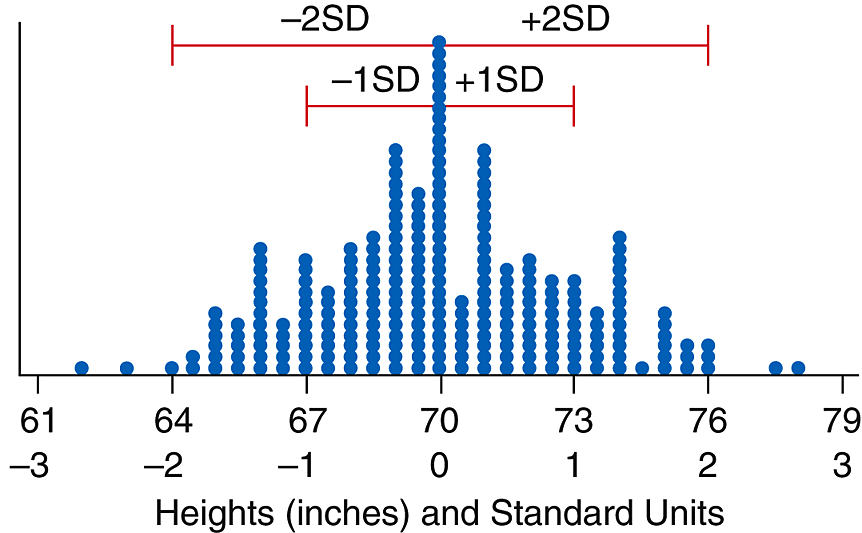
\includegraphics[width=0.6\linewidth]{images/math211_figure_3p12}
  \end{center}
  \pagebreak

  \begin{ex*}
    Maria scored 80 out of 100 on her first stats exam in a course and 85 out of 100 on her second stats exam. On the first exam, the mean was 70 and the standard deviation was 10. On the second exam, the mean was 80 and the standard deviation was 5.

    On which exam did Maria perform better when compared to the whole class?
  \end{ex*}

  \pagebreak
\end{document}
